\documentclass{sig-alternate}

\usepackage{graphicx} 
\usepackage{subfigure}
\usepackage{paralist}

\usepackage{hyperref}

\usepackage{url}
\usepackage{booktabs}

\usepackage[usenames,dvipsnames]{xcolor}
\usepackage{tikz}
\usetikzlibrary{positioning, calc}

\usepackage[draft,nomargin,footnote]{fixme}

\graphicspath{{figs/}}

\usepackage{xspace}
\newcommand{\eg}{\textit{e.g.}\xspace}
\newcommand{\etal}{\textit{et al.}\xspace}
\newcommand{\ie}{\textit{i.e.}\xspace}
\newcommand{\etc}{\textit{etc.}\xspace}
\newcommand{\vs}{\textit{vs.}\xspace}

\begin{document}

% if need info about conference :
%\conferenceinfo{WOODSTOCK}{'97 El Paso, Texas USA}

\title{CoWriter : Case Studies}


\author{Alexis Jacq$^{1,2}$, S\'everin Lemaignan$^1$, Fernando Garcia$^1$, Pierre Dillenbourg$^1$, Ana Paiva$^2$\\
$^1$CHILI Lab, \'Ecole Polytechnique F\'ed\'erale de Lausanne, Suisse,\\
$^2$Instituto Superior T\'{e}cnico, University of Lisbon, Portugal}


%   \author{
%   % 1st. author
%   \alignauthor
%   Alexis Jacq\\
%       \affaddr{EPFL}\\
%       \affaddr{IST}
%   % 2nd. author
%   \alignauthor
%   Severin Lemaignan\\
%       \affaddr{EPFL}
%   \and
%   % 3rd. author
%   \alignauthor Fernando Garcia\\
%       \affaddr{EPFL}
%
%   \alignauthor Pierre Dillembourg\\
%       \affaddr{EPFL}
%
%   \alignauthor Ana Paiva\\
%           \affaddr{IST}
%    }


\date{date comes here}


\maketitle
\begin{abstract}
Abstract comes here
\end{abstract}

\keywords{robot-supported educative activitiy, handwriting learning, learning
by teaching}

\section{Introduction}
% -> A new hri field
% -> What as been done before
% -> what is new here

%   \begin{figure}
%       \centering
%       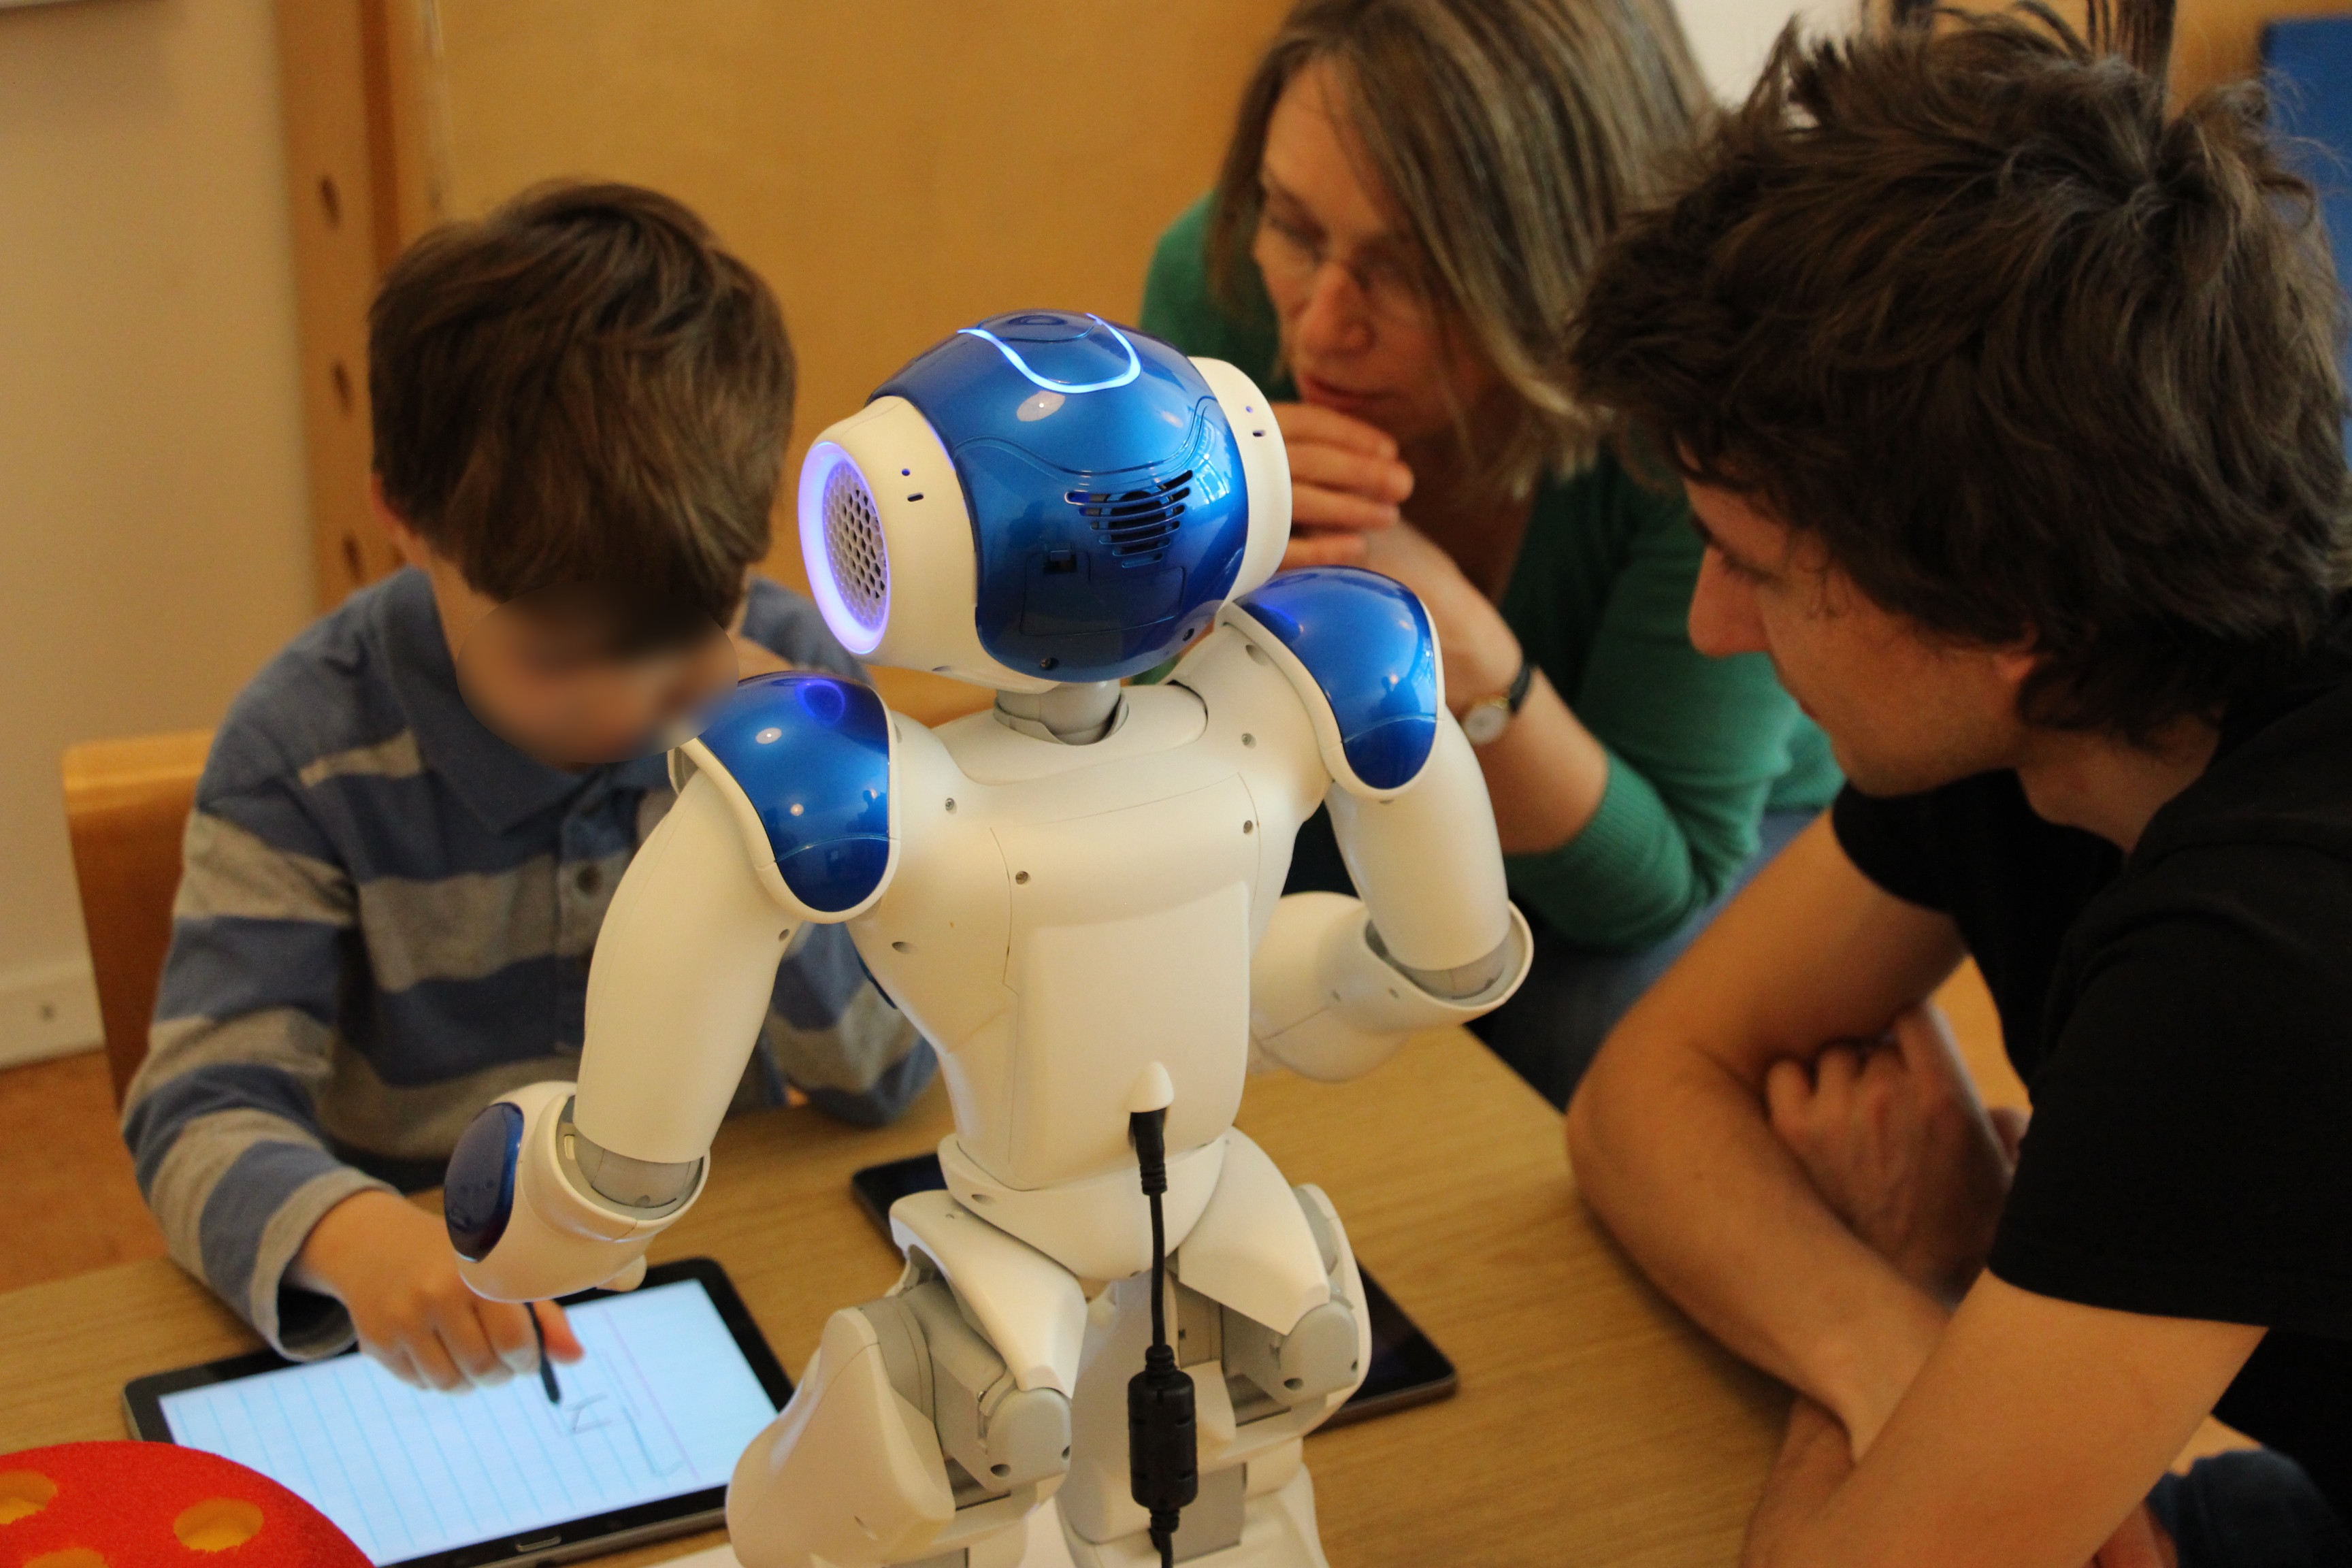
\includegraphics[width=0.9\linewidth]{henry}
%       \caption{Henry teaching Nao how to write numbers, with the help of an occupational therapist.}
%       \label{fig:henry}
%   \end{figure}

\section{The CoWriter activity}
\subsection{Children teach handwriting to the robot}
\subsection{Our approach}

\subsection{Learning and generating letters}

\subsection{robotic implementation}

\section{case 1 : Diego}
\subsection{Context}
Diego is a five years old child. Her mother told us he had difficulties learning
to write at school, particulary in drawing cursive letters. Before experiments,
she provided us with a homework of Diego to show explicitly his handwriting
level (fig). 

From our perspective, Diego is shy and quiet. He suffers from a poor
self-esteem much more than any actual trouble in writing.

\subsection{Questions}

The CoWriter activity needs a child engaged as interaction leader. 
In this study we consider the problem of long-term interactions: is it possible to
sustain this engagement over several one-hour sessions?

%   \begin{figure}
%       \centering
%       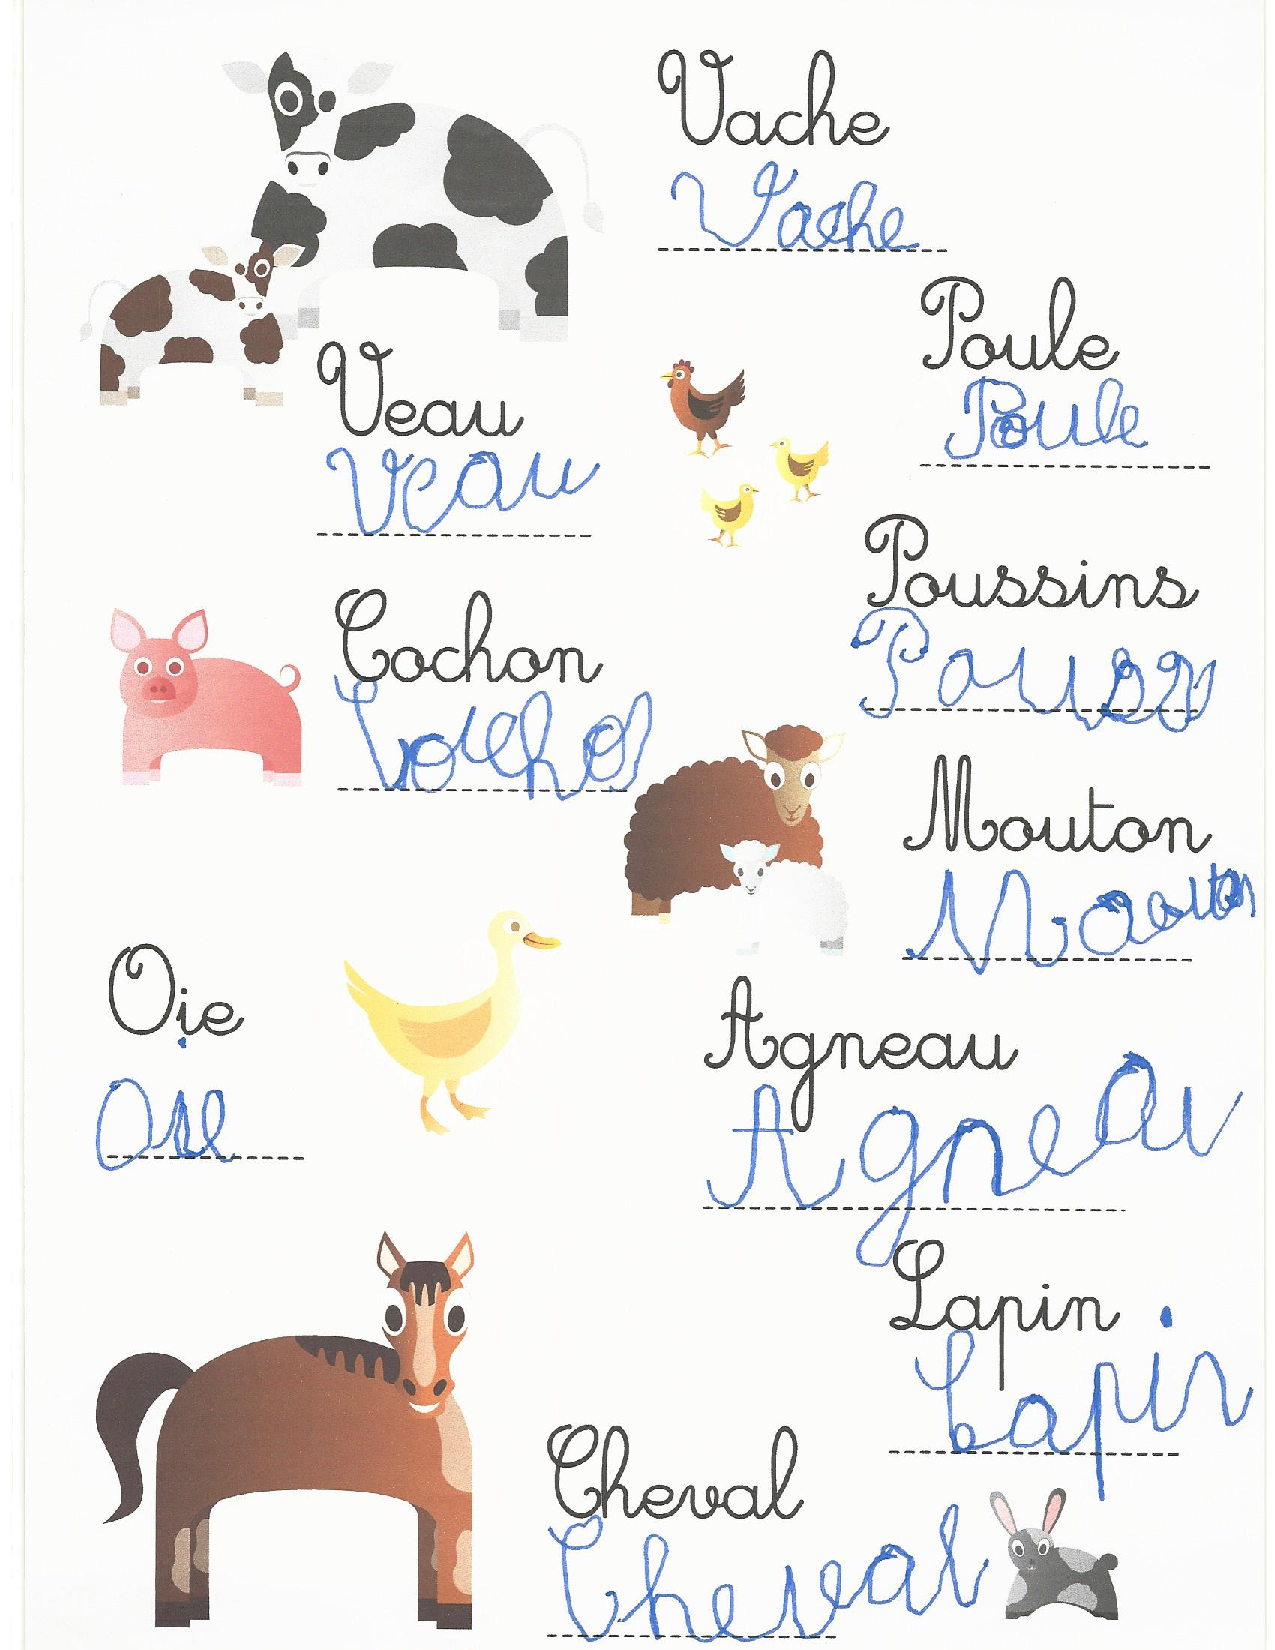
\includegraphics[width=0.9\linewidth]{diego_start}
%       \caption{Homework performed by Diego before the experiment. It gives an
%       overvew of his starting level in handwriting.}
%       \label{fig:diego_start}
%   \end{figure}

%   \begin{figure}
%       \centering
%       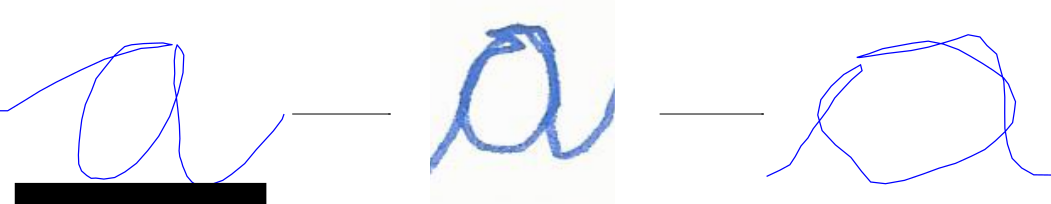
\includegraphics[width=0.9\linewidth]{3a}
%       \caption{Letter deformation along an eigenvector. \emph{Left} : the non-deformed
%           letter (origin of the eigenspace). \emph{Middle} : the actual Diego's
%           deformation (from figure~\ref{fig:diego_start}). \emph{Right} : exaggerated
%   deformation along the eigenvector that encode Diego's mistake.} 
%       \label{fig:3a}
%   \end{figure}

\subsection{Experimental settings}

The experiment took place in our laboratory. Our goal was to provide Diego with
an environment that would enable him to sustain engagement over four sessions 
of one hour, one session per week. We decided 
to introduce an appealing scenario that justified the activity to the child
where a robot wants to learn handwriting. We used two Nao robots: a blue one 
(called Mimi) and an orange one (called Clem). Mimi was away for a 
scientific mission, and the two robots had to communicate by mails. But they decided to do it 
``like humans", with handwritten messages. While Mimi was good in handwriting, 
Clem had strong difficulties and needed the help of Diego.

The mission of Mimi consisted in the exploration of a mysterious hidden
base. Each week, just before the session, it was sending a postal mail contening
a picture, a curious object it found and a few handwritten words about its discoveries. 
The picture was representing itself exploring 
a dark room of the hidden base (that was actually our laboratory's workshop). 
The objects were 3D printed. In fact, there where puzzle pieces of a small 3D 
model of Nao robot but seen separately, it was not easy to guess it.

During the three first sessions, Clem (the other robot) was waiting for Diego
with the received mail. It let Diego take a look at the picture and the object,
and then it asked him to read the message.
Finaly, Diego figured out a response and helped the robot to write it.

The fourth and last session was set as a test: Mimi, the ``explorer'' robot,
had come back from its mission and it actually challenged Clem in
front of Diego: \emph{``I don't believe you wrote yourself these nice letters that I
received! Prove it to me by writing something in front of me!''} This situation
was meant to evidence the prot\'eg\'e effect: by judging the other robot's
handwriting, Mimi would implicitly judge Diego's skills as
teacher, and in turn, Diego's handwriting.

To complement the intrinsic motivation of helping a robot to communicate with another one, we
gradually increased the complexity of Diego's task to keep it challenging and
interesting (first week: demonstration of single letters; second week:
short words; third week: a full message -- Figure~\ref{fig:stimuli}).

Diego had to tell the robot what to write with small plastic letters (visible
behind the robot on Figure~\ref{fig:diego}). A third person was here to send
the formed word to the robot via the computer.

%   \begin{figure}
%       \centering
%       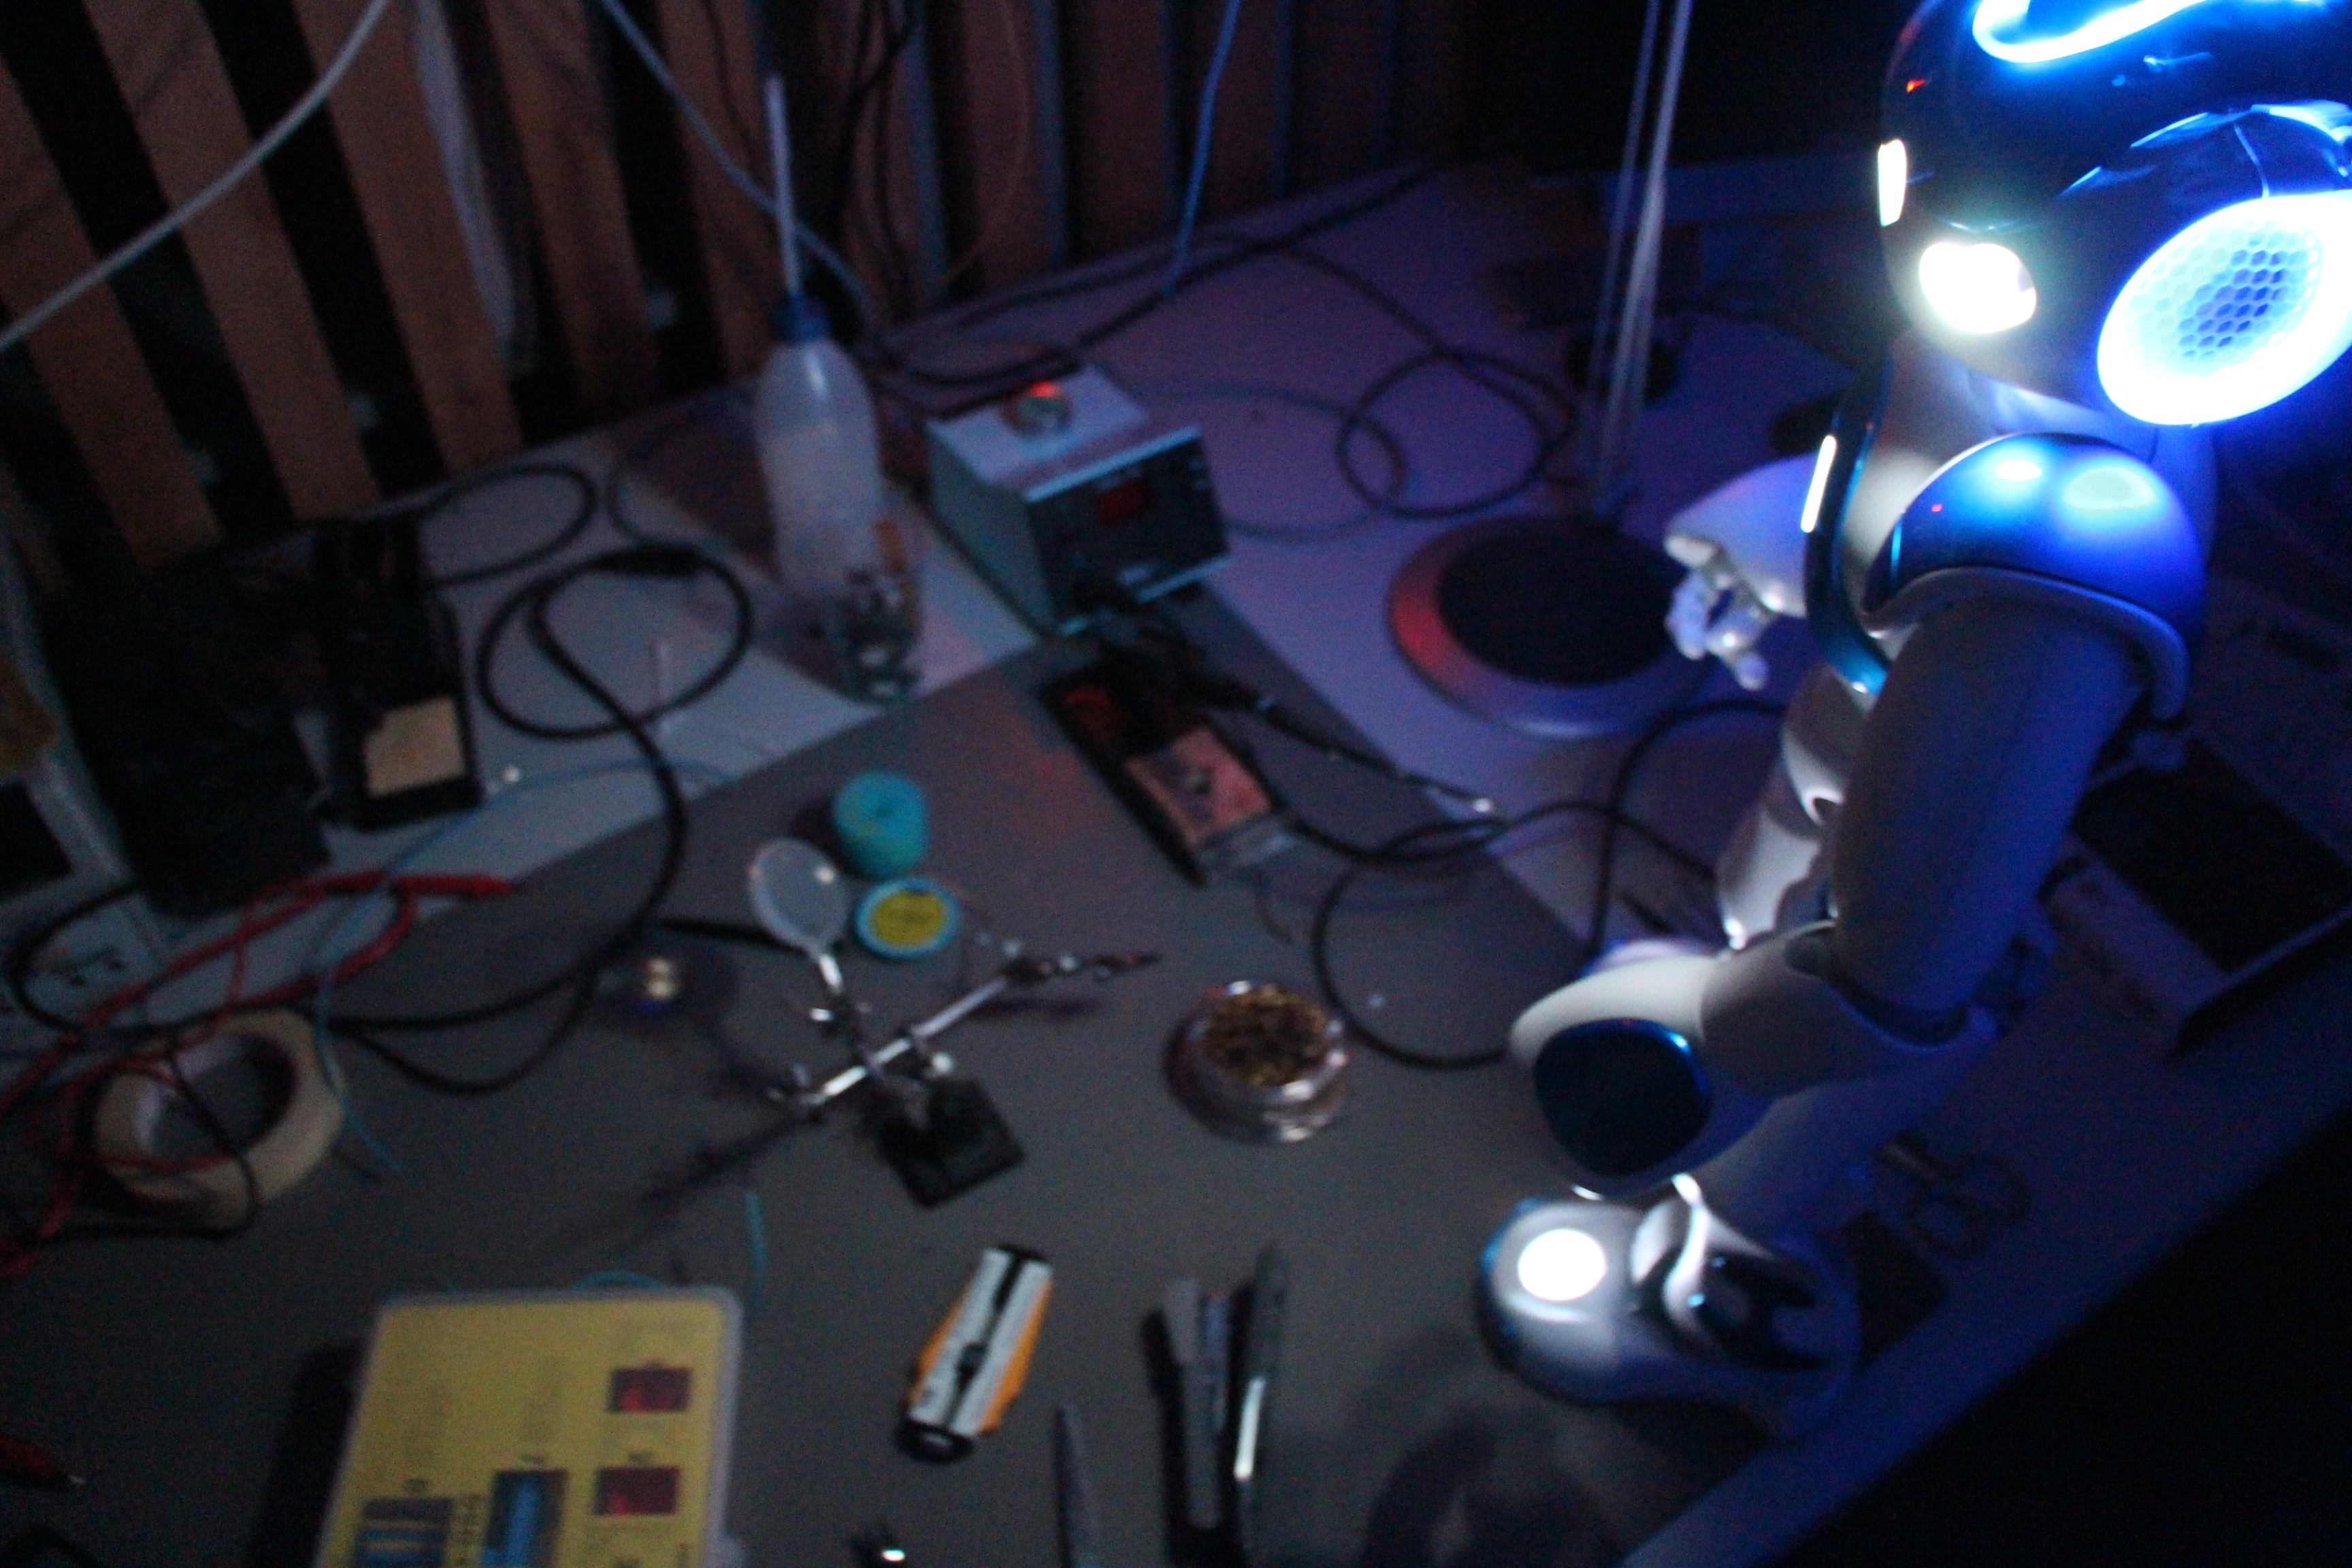
\includegraphics[width=0.9\linewidth]{mimi_mails}
%       \caption{Exemple of content of the mails sent by Mimi. A : pictures of Mimi exploring the
%           hidden base. B : some curious objects found by Mimi in the base. C :
%           few words about its adventures and discoveries.
%       }
%       \label{fig:mimi_mails}
%   \end{figure}


\subsection{Results}
Overall, Vincent provided 154 demonstrations to the robot, and he remained
actively engaged over the four weeks. The story was well accepted by Vincent and
he seriously engaged into the game. After the first week, he showed good
confidence to play with the robot and he built affective bonds with the robot
over the course of the study, as evidenced by some cries on the last session,
and several letters sent by him to the robot \emph{after} the end of the study
(one of them 4 months later) to get news. This represents a promising initial
result: we can effectively keep a child engaged with the robot for a relatively
long period of time (about 5 hours).

No conclusion can be drawn in terms of actual handwriting remediation: we did
not design this study to formally assess possible improvements.

However, as pictured on Figure~\ref{fig:stimuli}, Vincent was able to
significantly improve the robot's skill, and he acknowledged that he had been
able to help the robot: in that regard, Vincent convinced himself that he was
``good enough'' at writing to help someone else, and this is likely to have
positively impacted his self-esteem.



\section{case 2 : Henry}

\subsection{Context}

Henry, 5.5 years old child, is under the care of an occupational
therapist. He has been diagnosed with visuo-constructive deficits.
As an effect in writing activities, he was frequently performing random attempts and then was comparing
with the provided template. What is more, Henry is restless and careless: he
rarely pays attention to
advice, even to what he is doing when he is currently drawing, and he is
quickly shifting his attention from one activity to another.

Henry was working on number's allographs with his therapist. During a prior
meeting, the therapist provided us with a sequence of numbers
written by Henry~\ref{fig:henry_numbers}. Henry was sometime drawing
horizontally-inverted allographs, mainly for ``5".

\subsection{Questions}
This study focus on technical adaptations of the CoWriter activity for a 
child diagnosed with real writing deficits.
Our objective is to investigate small modifications of the activity adapted to
the troubles of Henry (visuo-constructive deficits and inattention) in order to
maintain him focused
on the activity during forty-minutes session, and to make the robot
evidently learning from his demonstrations.

\subsection{Experimental settings}
The experiment was conducted in the therapist's surgery  (four sessions 
spanning over 5 weeks). We assumed that a scenario like the one we used 
for Vincent was no longer relevant with Henry. We just introduced the robot 
and quickly said that it was seeking help to train for a robot handwriting contest.

In order to integrate our work with that of the therapist, we decided to adapt the 
CoWriter activity to teach numbers to the robot.

Since Henry was frequently drawing horizontally-inverted numbers, or even
unrecognizable allographs, the learning algorithm of the robot was converging to
meaningless scrawls. To fix this problem, we programmed the robot to refuse allographs that
were too distant to a reference with a threshold we arbitrary fixed. In that way,
the child was forced to take care on what he was providing to the robot as
demonstration. 

According to the therapist, it was easier for Henry to memorize the way to draw
a number if it was always done is the same order, \emph{e.g.} if the ``5" was always
drawn from the top-right tip down to bottom. Therefore we programmed the robot to
refuse as well a good allograph drawn in a wrong order. But in order to reassure Henry
about the right final allograph's shape, we made the robot able to recognize
such a drawing, and, when it occured, to tell the child something like:
\emph{``Oh, this is exactly the shape of the number I want to learn, but can you
show me how to draw it in the opposite order?"}

Also, to make
the robot's progresses evident, we modified the initialization step of the
learning algorithm to start with a roughly vertical stroke instead of a
deformed number (round 0 on Figure~\ref{learning_6_demos}).

In this setup, we added a second tablet with one button per number. It was used
by the child to chose a new number to teach to the robot. It also provided the
possiblity to enter letters or words, and to switch to another activity (the
robot telling a story).


\subsection{Results}
Despite his inattention, Henry was able to remain engaged in the activity during more than
forty minutes in each session. In total, 55 allographs out of 82 
provided by the child as demonstration were acceptable by the robot (with a
progressive improvement from 13 out of 28 in the first session up to 26 out
of 29 in the last session).

As soon as Thomas understood that the robot was only accepting well-formed
allographs, he started to focus on it and he would typically draw 5 or 6 times
the number before actually sending to the robot (the tablet let the children
clear their drawing and try again before sending it to the robot). According to
the therapist, it was the first time that Thomas would correct himself in such a
way, explicitly having to reflect on how \emph{another agent} (the robot) would
interpret and understand his writing. Figure~\ref{henry_progress} shows how
he gradually improved his demonstrations for some numbers, according to the
metric we used to make the robot accept/refuse trials.

Since the robot's handwriting started from a simple primitive (a stroke), each
time Thomas succeeded to have his demonstration accepted by it, the robot's
improvement was clearly visible (as measured in Figure~\ref{henry_distances}).
This led to a self-rewarding situation that effectively supported Thomas'
engagement.

\section{Automatic studies}

\subsection{Context}

The previous studies where adapted to children : we used a special
design for each case in order to sustain the child engaged in the activity.
This time, we conducted case studies with eight children trought a unique
design. Those children have in common difficulties to learn
cursive writing but the natures and intensities of those troubles are stricly
different from one child to another. Valentine (7 years), Alexandre (6.5) and
Jonathan (7) are under the care of an
occupational therapist. Enzo (8) and Matenzo (7) are repeating their school year
because of writing. Mona (6) and Adele (8) are bottom of their respective
classes in writing activities. Nathan (7) is under the care of a neurologist, and
has been diagnosed with specific language impairment. All of those children are
expected, given their school level, to have in mind the allographs of
cursive letters. 

\subsection{Questions}

The main purpose of this study is to test the ergonomy of CoWriter. As we
introduce the robot, we dont
provide children with any scenario and give to them minimal explanations. Then
we see how easily they take the role of the teacher and how seriously they try to help the robot.

\subsection{Experimental settings}

This experiment took place in the coffee room of a therapists shared surgery
in Normandie, France. Over two weeks, each child came three time for one-hour
session, except Adele and Mona who just did one session. A facilitator was here
just to explain the rules of the game and tablets usage. As for Henry, the child
had two tablets : one to choose a word (or a single letter) to teach, and one
used by both the child and the robot to write. Sometime, if the child asked for,
we provided him with allograph's template. 

The starting point of the robot's writing was the same for all children: we
used middle point between simple vertical strokes and letters. For this study,
we wanted the robot to be only influanced by the demonstrations provided the
child, so we did not projected allographs in an eigenspace. The generated
trials of the robot where directly the middle way between demonstration and
last state in cartesian space. 

We added two buttons on the tablet  interface. One green with a thumb up, and
one red with a thumb down. Those buttons could be used by children to evaluate the
robot (the green one was for rewards while the red one was for punishment). By
this way, we could mesure the perception of
the robot by the child: the more the child used evaluation buttons, the more he
was playing the teacher, judging the robot instead of himself. It becomes
possible to estimate if a child is playing seriously given correlation between
his evaluation and robot's actual progression.


\subsection{Results}

All children maintained their engagement during the full sessions. They provided
in average 42 demonstrations per session. All children used evaluation buttons and
had preference to reward the robot (at the end, 99 rewards was accorded to the
robot for 33 punishments). 

Since sessions took place over only two weeks, we did not studied possible
handwriting remediation in children. 

We focused on correlation between children's evaluations and robot's progression.
We estimated robot's progression as the difference between a starting score
(score of the first robot's try when children has chosen a new word/letter to
work on) and the current robot's score (after beeing taught by the child). We call score the average of euclidian
distance between robot's try and reference allograph over all letter of the
word. Those references for letter allographs where beforehand drawn by
us, taking inspiration in education.com cursive letters templates
(http://www.education.com/slideshow/cursive-handwriting-z/). Let $P_i$ be the
estimated progression of the robot at time $ i$. Of course, if the child
chose to switch to a new word at time $ j$ , we got $ P_{j}=0$ and obviously $
P_0=0$.
To mesure how significant a child was rewarding the robot when it was
progressing, we generated 10000 times the same number of reward/punishment
but accorded at random times. Let $ R_i^n$ be the nth generated evalutation at
time $ i$ ($ R_i^n = 0$ if
no evaluation occured at time $ i$ , $ R_i^n=1$ if a reward occured at time
$i$ and $R_i^n=-1$ if a punishment occured at time $i$), and $\overline{R}_i$ be the
actual evaluation at time $i$. For each nth generated sequence of evauation, we
compute a score of evaluation: $$ S^n = \sum\limits_i{R_i^n P_i}$$ 
Then we can estimate the p-value $p$ of the actual score: $$ \overline{S} =
\sum\limits_i{\overline{R}_i P_i}$$ 
given the distribution of the generated scores $\left(S^n\right)_n$, assumed to
be gaussian: 
$$p(\overline{S}) = 1-\phi{\left(\frac{\overline{S}-\mu}{\sigma}\right)}$$
where $\phi$ denotes the cumulative distribution function of standard normal
distribution, $\mu$ the mean and $\sigma$ the deviation of the generated 
scores $\left(S^n\right)_n$. 
As a result, we found that 5 of the 8 children obtained a score of evaluation
significantly hight ($p(\overline{S})<0.05$). We reported score of evaluation
p-values of each child in second-last column of Table~\ref{table:scores}.






\begin{table}
    \centering
    \begin{tabular}{|c|c|c|c|c|c|}
        \hline
        child & demo & pos & neg & p-value (robot) & p-value (child)\\ \hline
        valentine & 127 & 24 & 6 & 6.4e-05 & 2.3e-02\\ \hline
        enzo & 223 & 20 & 9 & 1.8e-01 & 5.8e-01\\ \hline
        matenzo & 131 & 10 & 3 & 1.5e-04 & 6.5e-04\\ \hline
        jonathan & 98 & 10 & 5 &  1.4e-01 & 6.6e-01\\ \hline
        nathan & 115 & 16 & 4 & 3.6e-06 & 2.7e-03\\ \hline
        alexandre & 83 & 10 & 3 & 8.5e-03 & 1.3e-00\\ \hline
        adele & 35 & 4 & 2 & 2.1e-02 & 1.3e-02\\ \hline
        mona & 40 & 5 & 1 &  1.1e-00 & 2.3e-01\\ \hline
    \end{tabular}
    \caption{results of evaluation. demo : number of demonstrations provided by
        the child over all session. rew : number of rewards accorded by
        the child. pun : number of punishments. p-value (robot) : how
        significant are the evaluation corresponding to robot's progression. p-value
    (child) : how significant are the evaluation corresponding to child's own progression.}
    \label{table:scores}
\end{table}


\section{Discussion}

\section{Conclusions}

\bibliographystyle{abbrv}
\bibliography{cowriter} 
\end{document}
